% 独自のコマンド

% ■ アブストラクト
%  \begin{jabstract} 〜 \end{jabstract}  :日本語のアブストラクト
%  \begin{eabstract} 〜 \end{eabstract}  :英語のアブストラクト

% ■ 謝辞
%  \begin{acknowledgment} 〜 \end{acknowledgment}

\newif\ifjapanese

\japanesetrue  % 論文全体を日本語で書く(英語で書くならコメントアウト)

\ifjapanese
  \documentclass[a4j,twoside,openright,11pt]{jreport} % 両面印刷の場合。余白を綴じ側に作って右起こし。
  % \documentclass[a4j,11pt]{jreport}                  % 片面印刷の場合。
  \renewcommand{\bibname}{参考文献}
  \newcommand{\acknowledgmentname}{謝辞}
\else
  \documentclass[a4paper,11pt]{report}
  \newcommand{\acknowledgmentname}{Acknowledgment}
\fi
\usepackage[dvipdfmx]{graphicx}
\usepackage[dvipdfmx]{color}
\usepackage{thesis}
\usepackage{ascmac}
\usepackage{graphicx}
\usepackage{multirow}
\usepackage{url}
\usepackage{latexsym}
\usepackage{here}
\usepackage{listings,jlisting}

\lstset{%
  language={C},
  basicstyle={\small\ttfamily\footnotesize},%
  breaklines=true,%
  identifierstyle={\small},%
  commentstyle={\small\itshape},%
  keywordstyle={\small\bfseries},%
  ndkeywordstyle={\small},%
  stringstyle={\small\ttfamily},
  frame={tb},
  breaklines=true,
  columns=[l]{fullflexible},%
  numbers=left,%
  xrightmargin=0zw,%
  xleftmargin=3zw,%
  numberstyle={\scriptsize},%
  stepnumber=1,
  numbersep=1zw,%
  lineskip=-0.5ex%
}
\bibliographystyle{jplain}

% ファイル綴じ用余白設定
% 左右対称にしたいので一旦コメントアウト
% \bindermode  

% 日本語情報(必要なら)
\jclass  {修士論文}                             % 論文種別
\jtitle  {HypAR Touch: NFCとwikiを利用したAR/VRナビゲーションシステム}      % タイトル。改行する場合は\\を入れる
\juniv   {慶應義塾大学大学院}                   % 大学名
\jfaculty{政策・メディア研究科}                 % 学部、学科
\jauthor {左治木 隆成}                            % 著者
\jhyear  {2}                                   % 平成○年度
\jsyear  {2020}                                 % 西暦○年度
\jkeyword{AR、ナビゲーション、NFC、Wiki、ハイパーリンク}       % 論文のキーワード
\jproject{} % プロジェクト名
\jdate   {2021年1月}

% 英語情報(必要なら)
\eclass  {Master's Thesis}                          % 論文種別
\etitle  {HypAR Touch: AR/VR navigation system using NFC and wiki}      % タイトル。改行する場合は\\を入れる
\euniv   {Keio University}                          % 大学名
\efaculty{Graduate School of Media and Governance}  % 学部、学科
\eauthor {Ryusei Sajiki}                                % 著者
\eyear   {2020}                                     % 西暦○年度
\ekeyword{AR, Navigation, NFC, Wiki, Hyperlink}          % 論文のキーワード
\eproject{}               % プロジェクト名
\edate   {January 2021}


\begin{document}

\ifjapanese
  \jmaketitle    % 表紙(日本語)
\else
  \emaketitle    % 表紙(英語)
\fi

% ■ アブストラクトの出力 ■
%	◆書式:
%		begin{jabstract}〜end{jabstract}	:日本語のアブストラクト
%		begin{eabstract}〜end{eabstract}	:英語のアブストラクト
%		※ 不要ならばコマンドごと消せば出力されない。



% 日本語のアブストラクト
\begin{jabstract}
NFC技術をARの正確な位置測位とコンテキスト情報の取得に活かしつつ、AR情報の管理にWikiの手法を取り入れたARナビゲーションシステム、「HypAR Touch」を提案する。
モバイル端末によるARナビゲーションは近年普及し始めたが、(1)立ち上げるまでのインタラクションが面倒、(2)位置測位の方法によって精度や用途が大きく限られる、(3)情報の登録・編集が面倒、(4)関連情報を参照・管理することができていないなどといった問題が存在する。
HypAR TouchではNFC技術を利用することで正確な位置測位やコンテキスト情報の取得を可能とする。
さらに、AR情報の管理にWikiを採用することでハイパーリンクから関連する情報を簡単に参照管理することができる。
これによってARナビゲーションの問題点が解決されるだけでなく、リンクを使ったより探索的な使い方が可能になる。
本論文ではHypAR Touchの設計や実装、その応用例について述べ、研究の発展性について考察する。
\end{jabstract}



% 英語のアブストラクト
\begin{eabstract}
We propose \textit{HypAR Touch}, an AR navigation system that utilizes NFC technology for accurate positioning and contextual information acquisition in AR while incorporating Wiki methods for AR information management. 
AR navigation using mobile devices become popular in recent years, but there are problems such as (1) cumbersome interaction to start up, (2) accuracy and applications are greatly limited depending on the location positioning method, (3) registration and editing of information is cumbersome, and (4) reference and management of related information is not yet available. 
HypAR Touch uses NFC technology to enable accurate positioning and acquisition of context information. 
Furthermore, by adopting a Wiki for managing AR information, related information can be easily referenced and managed through hyperlinks. 
This not only solves the problem of AR navigation but also allows for a more exploratory use of links.
This paper describes the design and implementation of HypAR Touch and its applications and discusses the development potential of the research.
\end{eabstract}
  % アブストラクト。要独自コマンド、include先参照のこと

\tableofcontents  % 目次
% \listoffigures    % 表目次
\listoftables    % 図目次

\pagenumbering{arabic}

\chapter{序論}
\label{chap:introduction}


本章では本研究の動機と目的、および本論文の構成について述べる。

\newpage


\section{研究の動機}
\label{motive}

拡張現実感(AR : Augmented Reality)によるヘルプ・ナビゲーションの歴史は長く、早いものでは1990年代から存在している。
またARにはヘッドマウントディスプレイを使うものと携帯端末のカメラを通した映像に情報を付加するものが存在するが、後者は近年のスマートフォンの普及と高性能化により利用環境が整って来ている。
しかし既存のARナビゲーションシステムには以下のような問題点があり、ARが汎用的なヘルプ・ナビゲーションシステムとして利用されていない現状がある。

\begin{itemize}
  \item 環境を問わず正確で安価に位置測位をすることが難しい
  \item 表示する情報の登録・編集が煩雑で参照や管理が面倒
  \item 案内を起動するまでの負荷が高い
\end{itemize}

一方でARでも頻繁に扱われるテキストや写真、地図などのマルチメディア情報は計算機の進歩とwebの発展とともに以下のような進化を遂げた。

\begin{itemize}
  \item 他の文書への参照を実現するハイパーリンクと、それを内包した文書であるハイパーテキストが登場した
  \item Webの普及によって様々なメディアにハイパーリンクを経由して手軽にアクセスできるようになった
  \item webからアクセス可能な地理情報システムが登場し地理情報の紐付けが用意になった
  \item コラボレーションツールであるWikiが複数人による共同編集を可能にし、知見の共有を実現した
\end{itemize}

さらにモバイル端末の高性能化により多くの端末で近距離無線通信(NFC : Near Field Communication)による非接触タグの読み書き機能が搭載されるようになっている。
NFCによる非接触タグには以下のような利点が存在する。

\begin{itemize}
  \item タグ側に電力を必要とせず、小型化できるためタグを設置する場所や物を選ばない
  \item 個別のIDやURL情報を記録するには十分な記憶容量を持つ
  \item 読み取り側で検知した時の動作をある程度規定できる
\end{itemize}

このような利点はヘルプシステムやナビゲーションシステムに利用するにあたって非常に有用なものであると考える。
\\
本研究ではNFCタグの利点をARの正確な位置測位とコンテキスト情報の取得に活かしつつ、AR情報の管理にWikiの手法を取り入れたシステムを開発し、既存のARナビゲーションシステムが抱える問題点を解決した。

\section{研究の目的}
本研究では、第\ref{motive}節で述べたARナビゲーションシステムが持つ問題点を解決するARナビゲーションシステム「HypAR Touch」の構築を目的とする。


\section{本論文の構成}

本論文は以下の8章で構成される。

第\ref{chap:background}章では、本研究の背景をより詳細に分析し、既存システムの問題点を整理する。

第\ref{chap:design}章では、本論文で提案するシステムの基本構成と使い方について述べる。

第\ref{chap:implementation}章では、本論文で提案するシステムの詳細な実装について述べる。

第\ref{chap:usage}章では、本論文で提案するシステムの利用例を紹介する。

第\ref{chap:relatedResearch}章では、関連する研究を紹介し、それらの特徴や本研究との関連を述べる。

第\ref{chap:consideration}章では、筆者による運用経験やユーザーからのフィードバックをまとめ、本論文で提案するシステムの有効性と問題点について述べる。

最後に、第\ref{chap:conclusion}章で本論文のまとめと結論を述べる。  % 本文1
\chapter{研究背景}
\label{chap:background}

本章では既存のARナビゲーションシステムの現状と、その問題点を整理する。

\newpage


\section{ARによるヘルプ・ナビゲーションシステム}
ARによる表示をヘルプやナビゲーションシステムに利用する研究はは90年代はじめから存在する。
初期の有名な例としてはプリンタのメンテナンス情報をARで表示するプロトタイプである、KARMA\cite{10.1145/159544.159587}や大学構内の案内をARで表示するナビゲーションシステムであるA Touring Machine\cite{629922}が挙げられる。
これらはヘッドマウントディスプレイを利用したものであるが当時のヘッドマウントディスプレイは非常に大型で性能の限界もあり実用的とは言えないものであった。

その後2000年代になりモバイル端末が普及するとGPSと方位などの情報をもとにカメラを通して周囲の情報をディスプレイに表示するアプリケーションが現れるようになった。
代表的なものとしてWikitude\footnote{\textsf{https://www.wikitude.com/}}が挙げられる。


\section{ARによるヘルプ・ナビゲーションの現状}
\label{current}
ARによるヘルプ・ナビゲーションとして実用化しているシステムを紹介し、その現状を解説する。

\subsection{Google MapsのARナビ機能}
Google \footnote{\textsf{https://google.com}}は2018年のGoogleI/O 2018で自社の開発する地図アプリケーションGoogle Maps\footnote{\textsf{https://www.google.com/maps}} にAR機能が追加されることを発表し、翌2019年5月にARナビゲーション機能としてα版をリリースした。
この機能ではGPSによる位置情報や方位情報、カメラからの画像情報などをもとに図\ref{fig:googleMapAr}のようなAR表示での道案内を表示する事が可能である。
本アプリケーションはカメラで取得した周囲の景色による補正からかなり高精度なAR表示を提供するが、用途はあくまでもあくまでも目的地までの経路案内に限られている。
またGPSの届かいない場所やGoogleStreetViewなどに景色の登録がない施設では利用ができないと言うデメリットが存在している。

\begin{figure}[h]
  \begin{center}
      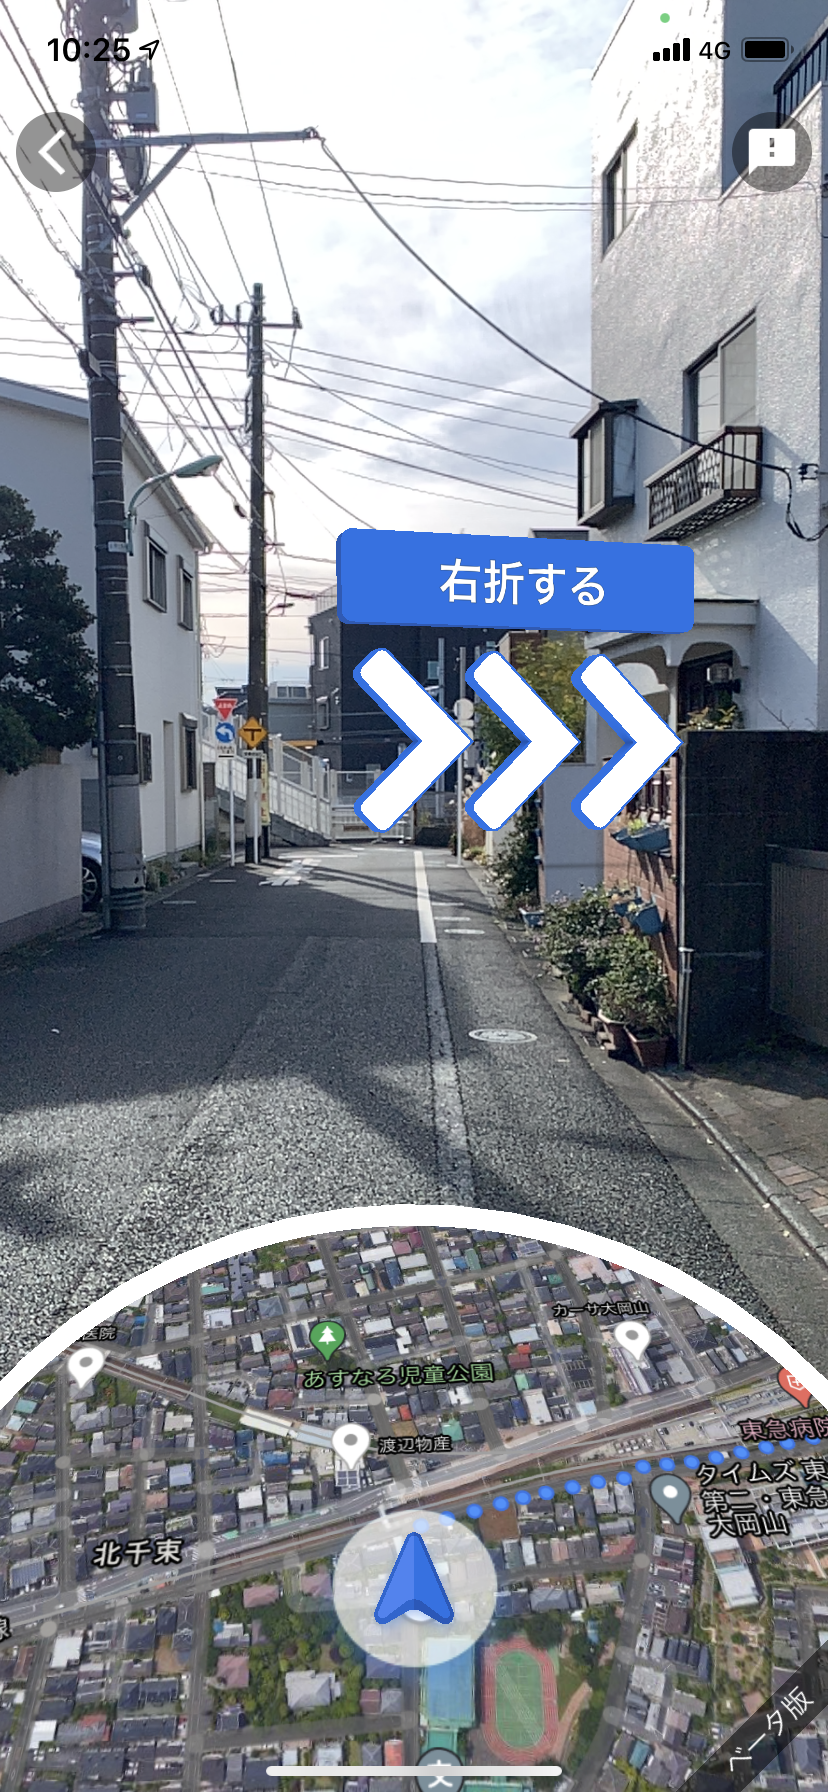
\includegraphics[width=60mm]{images/google-maps-ar-mode.png}
  \end{center}
  \caption{Google MapsでのAR表示} \label{fig:googleMapAr}
\end{figure}

\subsection{遺跡・史跡のARナビゲーションアプリ}
また日本国内の史跡ではマーカーベースのAR案内アプリケーションが複数存在しているしている。
殆どのものが史跡の近くにマーカーを設置し、そこから解説や当時の様子を再現したCGを描くというものである。
今回は一例として松山城址でのナビゲーションアプリである「攻略 松山城」\footnote{\textsf{https://www.cadcenter.co.jp/works/archives/98}}を紹介する。
このアプリは松山城の歴史や仕組みを解説するARナビゲーションアプリである。
図\ref{fig:matsuyama_marker}の専用のマーカーをアプリのカメラで読み込むことで図\ref{fig:matsuyama_ar}のように解説動画のリンクをを適切な位置に表示する。
このようなアプリの場合、表示したい場所ごとに図\ref{fig:matsuyama_marker}のような大きなマーカーを設置しなければならないと言う問題点がある。
また実際の運用を考えると専用のマーカーとアプリを利用しているため、多くのマーカー付近でアプリをダウンロードするための案内が別途必要になり、汎用性があるとは言い難い。


\begin{figure}[h]
  \begin{minipage}{0.5\hsize}
    \centering
    \includegraphics[width=70mm]{images/matsuyama_marker.jpg}
    \caption{専用のマーカー} \label{fig:matsuyama_marker}
  \end{minipage}
  \begin{minipage}{0.5\hsize}
    \centering
    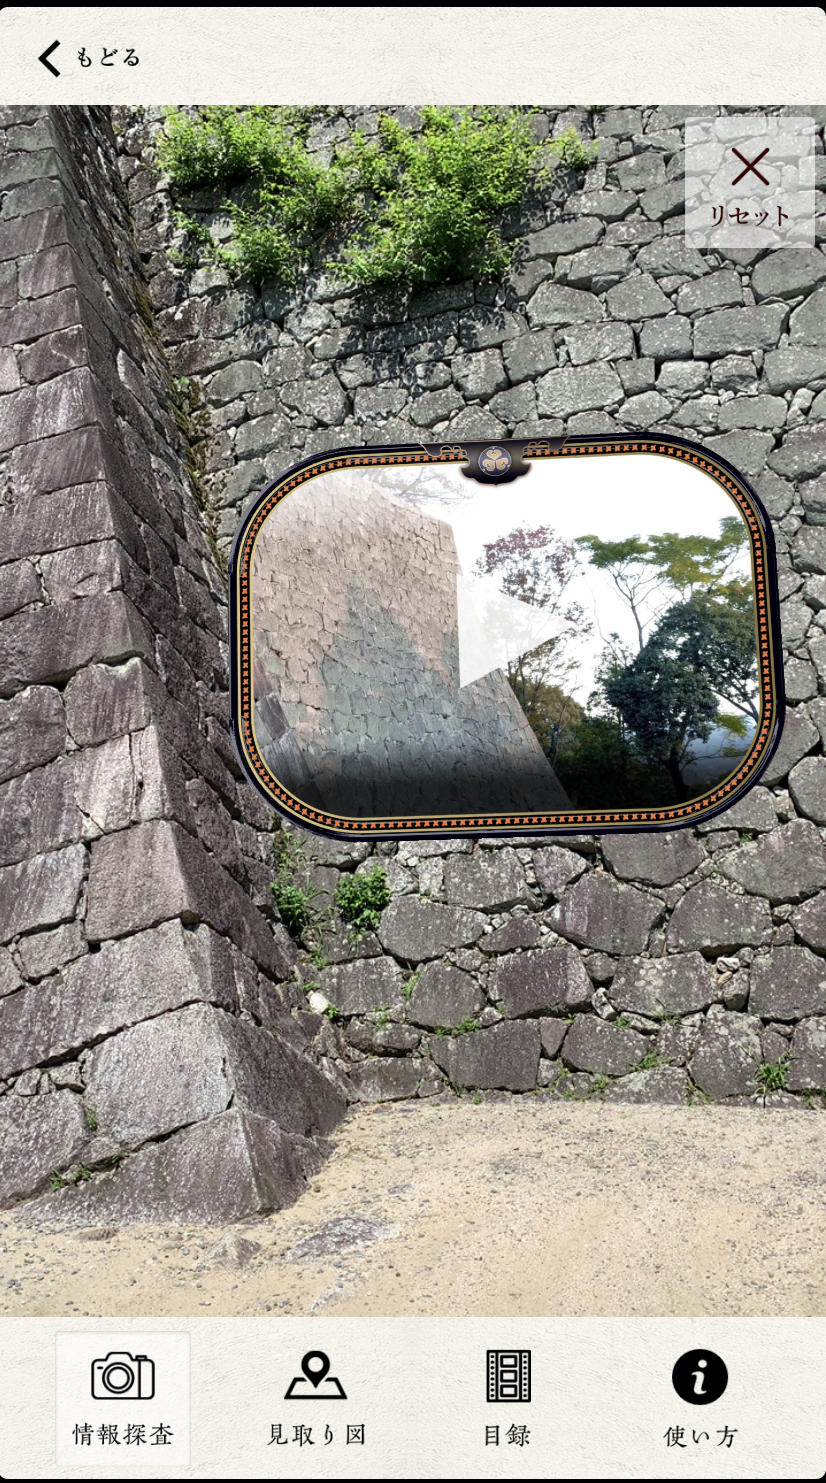
\includegraphics[width=60mm]{images/matsuyama_ar.png}
    \caption{ARでの案内} \label{fig:matsuyama_ar}
  \end{minipage}
\end{figure}


\section{ARによるヘルプ・ナビゲーションの問題点}
\label{problems}
前節で述べた現状を元に既存のARによるヘルプ・ナビゲーションシステムの問題点を整理する。
ARのナビゲーションシステムには以下のような問題点がある。

\begin{itemize}
  \item 立ち上げるまでのインタラクションが面倒
  
  前節の「遺跡・史跡のARナビゲーションアプリ」のようにマーカーベースのARナビゲーションでは設置された「マーカーを元にアプリを選択」、「起動」、「カメラでマーカーを中心に収める」という3ステップが必要になる。
  GPSと方位情報から位置測位を行うアプリケーションの場合、このような手順は必要ないが後述するように精度や用途か限られるという問題がある。
  
  \item 位置測位の方法によって精度や用途が大きく限られる
  
  ARでのナビゲーションを行う際に多く用いられる位置測位の方法は、(1)マーカーを使うものと(2)GPSによるの座標検知と方位情報をあわせて利用するものの2通りに大別される。
  (1)の場合その場での精度は高いが、ある程度の距離からカメラで十分認識できるサイズのマーカーを設置する必要がある。
  (2)の場合特別な設備は必要ないが精度での疑問が残ることに加えGPS電波の届かない屋内での利用が限定される。
  前節で挙げたGoogle MapsのAR機能ではGPSや方位情報に加えGoogleが撮影した道路の画像を元に補正を行い、精度を挙げているが撮影されていない屋内での利用ができないという問題点は残る。

  \item 情報の登録・編集が面倒
  
  ARで単に目的の位置を表示したり、決め打ったデータを表示するARナビゲーションアプリは多いが、情報の登録や編集の簡易さに焦点を置いた物は少ない。
  ARでの表示したい情報は常に変化する可能性があり、増加していくことが予想される中で一般ユーザが気軽に情報を登録編集できる環境を整えることは急務と言える。

  \item 関連情報を参照・管理することができていない
  
  ARでの表示する情報が増えるにしたがってそれらを互いに参照したり、ドメインごとに管理するニーズは高まっていくと考える。
  しかしながら既存のアプリケーションではARで表示した情報同士を互いに参照して関連情報を表示したり、特定の分野でフィルターすることが難しい。

  \item 汎用性のあるアプリケーションがない
  上記のように「情報の登録・編集が面倒」、「関連情報を参照・管理することができていない」という問題点から特定の目的や分野に限ったARナビゲーションアプリは存在するものの、分野や目的を横断した汎用的ARナビゲーションは開発されていない。
  その結果目的や施設ごとにアプリケーションをユーザ側で切り替える必要があり、ARナビゲーションアプリが増えるほどユーザの負担は大きくなる。
  さらに目的や施設ごとにアプリケーションと情報が独立してしまうことで分野を横断したつながりを表現できないという問題点も生まれる。

\end{itemize}


\section{テキストや画像の進化}
前節で述べたとおりARによるヘルプ・ナビゲーションには課題が多いが、ナビゲーションに利用しているテキストや画像などのメディアは計算機の進化とともに多くの問題点を克服している。

計算機上で利用されているテキストは、文字から内容を検索することが可能なため文書の参照や管理が格段に行いやすく、あらゆる文書の作成が電子化されたテキストに置き換えられるようになった。
またWebやハイパーリンク等の技術によってより参照しやすくなったほか、別の文書を引用する等の再利用が可能になった。
さらにハイパーリンクを含んだ文書を手軽に作成・編集できるWiki\cite{Leuf2001TheWW}が登場したことでより柔軟・活発なテキストによる知見の共有や情報の再利用が実現された。

同様に画像や地図などのメディアも電子化とwebの進歩により参照や管理が格段に行いやすくなった。
SNSや画像の管理が行えるクラウドウェアの普及により誰しもが写真を撮影し容易にweb上にアップロード/公開することが可能になり、公開された画像はURLによって一意に参照することができることから画像の再利用性は大きく高まった。
またGoogle Mapsのように、地理情報システム(GIS : Geographic Information System)で誰でも検索・参照可能な形でWebに公開されることで位置情報や地理情報を参照することが容易になった。

このような文書以外のメディアの進化に合わせ、近年の文書作成システムやWikiシステムは画像/音声/動画/地図といったマルチメディアを自在に埋め込む機能を持っている。


\section{NFC技術とインタラクション}
ARでのナビゲーションシステムには自身の位置情報やその場のコンテキスト情報などが不可欠であり、一般的にそのような情報を瞬時に取得することは難しい。
一方NFCタグには以下のような特徴から実世界においてその場のコンテキスト情報や設置されたものの情報を記述するのに便利である。

\begin{itemize}
  \item 電源がいらない
  \item 非常に薄く、小型
  \item IDやURLなどを記録するには十分な記憶容量を持つ
  \item 一枚あたり10円前後と安価
\end{itemize}

近年では多くのモバイル端末にNFCタグの読み取り機能が搭載されており、一般的なNFCタグであれば誰でも書き込まれた情報を瞬時に読み取ることができる。
さらに書き込むデータ形式によっては、モバイル端末でNFCタグの読み取るだけでwebページを開いたり、アプリを起動することが可能である。

このようなNFCタグの特徴は、既存の用途である決済や在庫管理、家電操作などに加えナビゲーションシステムを補助するシステムとして有効であると考える。

また一般的なNFCタグは読み取る際に、読み取る機器をNFCタグにかなり近づける必要がある。
この技術的制約は一般的にデメリットとして捉えられがちであるが、一方でNFCタグを読み取ったタイミングでのユーザの持つ端末の位置はNFCタグとほぼ接していると確定できることになる。
つまりNFCタグに位置情報をもたせれば非常に少ない誤差でユーザの持つ端末をの位置を確定できることになる。
この特徴は第\ref{problems}節で述べた問題点の1つであるNFCの位置測位の問題を解決するものである。


\section{まとめ}
ARをナビゲーションとして利用するアイデアは以前から存在し、実用段階に来ているプロダクトも増えてきている。
ただし第\ref{problems}節に上げた問題点を解決できていないため、汎用的なヘルプ・ナビゲーションとして利用されるに至っていない。
一方でナビゲーションに利用しているテキストや画像などのメディアは計算機上で積極的に応用されており、ハイパーリンクやWiki等の技術によって参照や再利用がより行いやすくなった。
また近年多くのモバイル端末に搭載されているNFC技術には第\ref{problems}節であげた問題点の一部を克服する可能性がある。
したがってARの正確な位置測位とコンテキスト情報の取得にNFCの技術を利用しつつ、ARで表示する情報の管理にWikiの手法を取り入れることで第\ref{problems}節に挙げた問題を解決できると考える。
次章では上記のようなARナビゲーションシステムが持つ問題点を解決し、次世代のARナビゲーションシステム「HypAR Touch」を提案する。  % 本文2
\chapter{設計}
\label{chap:design}

本章では次世代のARナビゲーションシステム「HypAR Touch」の要件と設計について述べる

\newpage

\section{要件}
前章で整理したARナビゲーションシステムの問題点を踏まえた上でHypAR Touchシステムの要件を整理する。
\begin{enumerate}
  \item 手軽なインタラクションでアプリケーションの起動と位置測位ができる。
  \item 周囲のコンテキストを簡単に指定できる。
  \item ARでの表示情報を容易に登録・編集できる。
  \item ハイパーリンクを利用し、関連情報を参照・管理することができる。
\end{enumerate}
これらの要件を満たすARナビゲーションシステムは、NFCをタッチするインタラクションとハイパーテキストの編集環境であるWikiの組み合わせによって実現できる。

\section{設計}
NFCを利用したインタラクションとWikiを採用することで前節に上げた要件を満たすことを説明し、本システムの設計を記述する。

\subsection{NFC技術の利用}
前章で述べた通りNFCタグの持つ様々な性質はナビゲーションシステムにとって有用である。
この性質を利用し、NFCタグのタッチからアプリの起動と位置測位を行うことで前節の要件1を満たすことができる。
またNFCタグに記録された情報から周囲のコンテキストを把握することで前節の要件2が達成される。

\subsubsection*{要件1:手軽なインタラクションでアプリケーションの起動と位置測位ができる}
NFCタグによるインタラクションにはカメラでマーカーを読み込むインタラクションなどと比べて以下のような優位性がある。
\begin{itemize}
  \item データの読み込みが非常に早い
  \item モバイル端末でアプリが起動していない状態でも読み込み可能である
  \item 周囲の明るさなどの環境要因に左右されず安定して読み込み可能である
\end{itemize}
このようなNFCタグによるインタラクションの特徴を利用し、HypAR Touchでは次のような動作を設計した。
\begin{enumerate}
  \item NFCタグに緯度経度・方位の情報を記録する。
  \item NFCタグへのタッチを契機にアプリケーションを起動する。
  \item NFCタグを読み取るには数センチ以内の距離で平行にタッチする必要があるため、モバイル端末の位置が確定する。
  \item 3での前提を元にNFCタグに記録された緯度経度・方位の情報から初期位置を算出する。
  \item アプリの起動後は4で設定した初期位置とモバイル端末の加速度センサによるデータを組み合わせ位置を算出する.
\end{enumerate}
これにより「NFCタグにタッチする」という手軽なインタラクションでアプリケーションの起動及び位置測位が実現できたことになる。

\subsubsection*{要件2:周囲のコンテキストを簡単に指定できる}
NFCタグには上記の特徴以外にも以下のような利点がある。
\begin{itemize}
  \item 小型である
  \item 電源がいらない
  \item 情報を埋め込める十分な容量
\end{itemize}
このような特徴は実世界に設置し周囲のコンテキスト情報を記録する媒体として非常に優れている。
本研究においてはNFCタグを利用し、緯度経度情報や方位の情報のみならず設置している物や場所に合わせた情報なども記録する。
また本システムは普及に向けた観点から、事業者やユーザーなどシステムに詳しくない一般人がタグを設置するを想定している。
そのためNFCタグを利用することには上記の理由に加え以下のような点からもメリットがある。
\begin{itemize}
  \item 1枚あたりのコストが十数円と非常に安価である
  \item 読み込み距離を担保できれば外見を気にすることがなく設置が楽である
\end{itemize}
本システムではこのような特徴を活かし、誰もがNFCタグを設置できるよう一意なIDを記録したNFCタグを配布し、
貼り付けた場所の情報をアプリから登録する方法を採用した。


\subsection{Wikiの利用}
Wikiはハイパーリンクを含んだ文書を手軽に作成・編集・管理できるツールである。
WikiシステムをAR情報の管理・編集ツールとして利用することで前節の要件3、4を満たすことができる。

\subsubsection*{要件3:ハイパーリンクを利用し関連情報を参照・管理することができる}
Wikiはハイパーリンクによってページ間にリンクを張ることができ、個々のページが高度に連携した文書群を作成することができる。
その結果適切にリンクが貼られていれば文書内のリンクを辿るだけで容易に関連情報を参照することが可能である。
このようなWikiの特徴はナビゲーションシステムにおける関連情報の提示に適しているといえる。

\subsubsection*{要件4:ARでの表示情報を容易に登録・編集できる}
現在多く使われるWikiシステムにはWeb上で内容を編集する仕組みが標準で備わっており、誰もが容易に内容を登録・編集することが可能である。
またハイパーリンクやタグの記述に加え、画像や動画といったメディアの参照・埋め込み機能に対応しているシステムも多い。
このように高機能な編集機能をもったWikiをARナビゲーションの情報源として利用することでAR情報を容易に登録・編集できる環境を実現する。

\begin{figure}[h]
  \centering
  \includegraphics[width=120mm]{images/wikipedia_edit.png}
  \caption{Wikipediaでの編集画面} \label{fig:wikipedia_edit}
\end{figure}

\subsection{NFC技術とWikiの併用}
上記のようなNFC技術とWikiの利点を組み合わせることで前節の要件5も満たすことができる。

\subsubsection*{要件5:広い分野の知見と用途を総合的に管理できる}
Wikiはハイパーリンクで情報を整理・参照するため、グループによる情報分類や階層的な情報の管理を必要としない。
したがってWikiでは異なる分野の情報をフラットに管理し、参照することができる。
実際ににWikiシステムを利用した百科事典であるWikipediaはあらゆる分野の情報を総合的に管理しながらも破綻なくシステムを運用している。
このようなWikiシステムをAR情報の管理に利用することで、分野を横断した知見の管理が可能になり、様々な用途に対応したナビゲーションシステムを作成できる。

Wikiシステムを利用すると広い分野の情報を一元的に管理することができるが、一方で自身の欲しい情報を探す際に手間となる事がある。
これを避けるためにNFCタグに記録されたコンテキスト情報を活用し検索・フィルタが可能なシステムを本研究では採用した。

これより広い分野の情報を一元的に管理できるWikiの利点を活かしながら様々な用途に対応したナビゲーションを提供する事が可能となる.



\section{まとめ}
本章では第\ref{chap:background}章で整理したARナビゲーションの現状と問題点を元に次世代ARナビゲーションシステム、HypAR Touchの要件を定義した。
さらに定義した要件はNFC技術とWikiシステムを組み合わせることで達成されることを提案し、その詳細を設計で示した。
次章では本設計を元に開発したHypAR Touchの実装とその機能を説明する。  % 本文3
\chapter{実装}
\label{chap:implementation}

本章では第\ref{chap:design}章で述べたシステムの設計を受け、HypAR Touchの実装について述べる。

\newpage

\section{アプリケーション構成}
HypAR TouchはARナビゲーションを表示するモバイルアプリケーション、AR情報やNFC情報を永続化しAPIを提供するサーバー、Scrapbox、Gyazo\footnote{\textsf{https://gyazo.com}},NFCタグで構成される(図 \ref{fig:application_structure})。

\begin{figure}[h]
  \centering
  \includegraphics[width=150mm]{images/application_structure.jpg}
  \caption{構成図} \label{fig:application_structure}
\end{figure}

\subsection{HypAR Touchアプリ}
HypAR TouchアプリはReactNative\footnote{\textsf{https://reactnative.dev/}}と呼ばれるフレームワークを利用して作成されたモバイル端末アプリケーションである。
ReactNativeはweb技術を利用し、マルチプラットフォームなネイティブアプリケーションを作成するためのフレームワークである。
このReactNative利用することでHypAR TouchアプリはAndroidとiOSの両方に対応したアプリケーションとなっている。

HypAr TouchアプリはNFCに記録された一意なidを取得し、そのidに紐付いた以下の情報を後述するHypAr Touchサーバーから取得する。
\begin{itemize}
  \item NFCタグの緯度経度
  \item NFCタグの設置される向き(0〜360度)
  \item 表示するAR情報の元となるScrapboxのプロジェクト名
  \item タッチした時に選択されているリンク情報
\end{itemize}
さらに取得したScrapboxのプロジェクト名をもとにHypAR TouchサーバーからARで表示する情報を取得する。
その上で取得したARの情報とNFCタグの緯度経度、NFCタグの設置された向きをもとに、各AR情報の位置を相対的に算出している。
また各AR情報には登録された位置付近で撮影されたパノラマ画像のURLが含まれている。
視点移動機能ではこのURLで登録された360度画像からVRのビューを作成している。

\subsection{HypAR Touchサーバ}
HypAR TouchサーバはNode.js\footnote{\textsf{https://nodejs.org/}}上で動作するWebアプリケーションとして実装されている。
HTTPリクエストを処理するWebアプリケーションフレームワークとしてExpress\footnote{\textsf{https://expressjs.com/}}を用い、
そのホスティング環境としてBaaS(Backend-as-a-Service)の1つであるHeroku\footnote{\textsf{https://www.heroku.com/}}を利用している。
HypAR TouchサーバはHypAR Touchアプリで利用するAR情報やNFCタグ情報を管理する役割をもっており、その機能は大きく4つに分けられる。

\begin{itemize}
  \item 対象となるScrapboxのプロジェクトをクロールし、AR表示に必要な情報を整理した上で永続化する。\\
  HypAR Touchサーバは指定されたScrapboxのプロジェクトを定期的にクロールし、位置情報やサムネイル画像のURL、リンク情報など、AR表示に必要な情報をまとめてデータベースに永続化している。
  これによりユーザがScrapboxに加えた変更がARでの表示に対応するようになっている。
  \\
  \item 登録されたNFCタグに関する情報を永続化する。\\
  NFCタグには一意なidが記録されており、それに紐づく形でタグの位置情報や向き、対象とするScrapboxプロジェクトなどの情報がこのサーバーに記録される。
  \\
  \item クロールした情報を元にパノラマ画像を生成し、Gyazoに保存した上でそのURLを記録する。\\
  第3章で記述した視点移動機能を実装するためにはARで表示する情報に加えて、記録された位置情報に最も近いところから撮影されたパノラマ画像が必要である。
  そのためHypAR TouchサーバではARで表示する情報ごとにGoogle Street ViewのAPI\footnote{\textsf{https://developers.google.com/maps/documentation/streetview/overview}}を利用してその地点からのパノラマ画像を生成している。
  また、画像の保存・永続化には後述するGyazoを利用しており、最終的にはGyazoに保存されたパノラマ画像のURLをARで表示する情報と合わせてデータベースに永続化している。
  \\
  \item 上記3つの情報を取得・追加・変更するAPIを提供する。\\
  HypAR Touchサーバは上記3つの情報を生成・永続化するだけでなく、HypAR TouchアプリからのAR情報取得やNFCタグの登録を受け付ける必要がある。
  そのためHypAR Touchサーバはこれらの情報を取得、追加、更新するAPIを提供している。

\end{itemize}

\subsection{Scrapbox}
Scrapboxは第3章で記述したとおり、AR表示するための情報を登録・編集するためのプラットフォームとして利用している。
Scrapboxはプロジェクト内のページリストと各ページの情報を取得するAPI\footnote{\textsf{https://scrapbox.io/help-jp/API}}を持っており、これを利用することでHypAR TouchサーバはScrapboxをクロールしている。

\subsection{Gyazo}
Gyazoは、パソコンのデスクトップ画面の一部をキャプチャしてWebにアップロードするツールおよび画像を保存する画像/映像専用のクラウドストレージサービスである。
Gyazoには十分な保存容量があり、画像のアップロード・取得等のAPIも揃っている。
そのため自身のサーバよりも安全に画像を管理可能なGyazoを本システムでのパノラマ画像の保存先として利用している。

\subsection{NFCタグ}
本システムで利用するNFCタグはモバイル端末のOSに関わらず、読み込めるタグ形式とデータフォーマットでなくてはならない。
そのため本システムではNFCタグとして最も普及しているISO/IEC 14443 TypeAに準拠したNFCタグを利用している。
また同様にNFC FORUMが策定したデータフォーマットであるNDEFを利用することでNFC機能を持つほとんどのモバイル端末に対応している。
NDEFのデータ形式には更に細かく、Text、URI、SmartPostermの3つのタイプが存在する。
このうちURIタイプで書かれたNFCタグは殆どのNFC対応スマートフォンでのバックグラウンド読み取りに対応している。
またAndroidとiOSにはディープリンクと呼ばれる特殊なURIからインストールされたアプリケーションを起動する機能が存在しており、そのURIの形式をCustom URL Schemeと呼ぶ。
Custom URL Schemeでは図\ref{fig:custom_url_scheme}のように起動するアプリの指定だけでなく、URIパラメータを利用して追加の情報を記述しアプリケーション側にその情報を渡すことが可能である。
このような特徴を踏まえ、本システムではNFCタグにCustom URL Schemeの形にしたURIをNDEFのURIタイプとして記録している。
これにより、モバイル端末でNFCタグにタッチするだけでアプリの起動及びタグIDの受け渡しが可能となる。


\begin{figure}[h]
  \centering
  \includegraphics[width=150mm]{images/custom_url_scheme.jpg}
  \caption{Custom URL Scheme} \label{fig:custom_url_scheme}
\end{figure}


\section{NFCによるキャリブレーション}
NFCタグによって行われる位置推定の仕組みについて解説する。
  % 本文4
\chapter{応用例}
\label{chap:usage}

本章では、HypAR Touchによって実現可能な応用例について述べる。

\newpage


\section{駅など公共施設での案内}
駅や空港などの比較的大規模な公共施設内ではGPSによる案内が利用できないことが多く、地図を提示するか矢印などによる案内表示が一般的である。
地図は設置できる場所に限りがあるだけでなく、位置関係が複雑な場合は地図を見ただけでその構造を理解することは難しく、目的地にたどり着くのが難しいという問題点を持つ。
また案内表示の場合、記述できる情報に限りがあり、必ずしも自分の目的地に沿う案内があるとは限らないという問題点がある。

一方本システムではARで目的地を直接提示(図:\ref{fig:ar_navigation_shonandai})するため地図の苦手な人への案内や複雑な構造の施設の案内において有用である。
また壁など設置された小さなNFCタグに触れるだけでその場所からの案内を開始できるため設置場所にこまることがない。
さらにNFCタグは一枚あたり十数円と安価であるため設置数とコストに困ることは少ないと言える。
またNFCタグに紐付いた情報により表示するAR情報のあるScrapboxプロジェクトとやハイパーリンクによるフィルターを指定できるので用途に特化した案内(図:\ref{fig:ar_navigation_exit})をすることも可能である。

\begin{figure}[htbp]
  \begin{minipage}{0.5\hsize}
    \centering
    \includegraphics[width=70mm]{images/wip2.jpg}
    \caption{案内の様子} \label{fig:ar_navigation_shonandai}
  \end{minipage}
  \begin{minipage}{0.5\hsize}
    \centering
    \includegraphics[width=70mm]{images/wip2.jpg}
    \caption{出口だけの案内} \label{fig:ar_navigation_exit}
  \end{minipage}
\end{figure}

\section{近隣施設の探索・推薦}
本システムの大きな特徴としてwikiを利用することにより情報を階層化せずに関連情報を探索できる点が挙げられる。
自分の興味のある近隣施設をリンクによって探索することが可能になっている。

例えば神保町で本システムを利用した場合、ウィンタースポーツ用品店を選択すれば、「スノーボード」「スキー」といったいったリンクが出現する。
ウィンタースポーツ用品店を周りたい場合はこれらのリンクを選択することでウィンタースポーツに関連する施設の情報を見ることができる。

またその後食事をを取りたくなった場合は同じタグにタッチし飲食店をクリックすることで「ラーメン」「カレー」等のリンクが出現し自身の食べたいものを絞り込みながら探索できる。
このように様々な施設の情報が混在していてもリンクをクリックしていくことで自分の求める情報を探索できるため、非常に拡張性の高いシステムになりうる。


\section{学習教材としての利用}
wikiはwikipediaに代表されるように膨大な史実や地理情報を整理し、記録するのに適したメディアであると言える。
本システムではwikiの各ページに位置情報を貼り付けるだけでARでの表示を実現できるためこのような地理情報を含む歴史や地理の教材として利用することが可能である。

例として京都などの史跡が多い地域でフィールドワークを行う際に利用することなどが考えられる。
学習者は各地にあるタグに触れるだけで周辺にある史跡の情報見ることができるだけでなく、選択した史跡の関連情報から他の史跡の情報や位置をARで見ることができる。
こうすることで自身の興味や学習対象に関連する史跡を効率よく回り、自身の知らない史跡を知る切っ掛けにもなると考える。

さらに本システムでは第3章で述べた通り現在地からのAR表示だけでなく選択されたAR情報の場所に視点を移動する事が可能である。
この機能によって実際の場所にいなくとも関連情報を元に視点を切り替えながら史跡を見ることが可能である。

\section{リンクを利用した柔軟な記法}
WIP


\section{まとめ}
本章では、本システムによって実現可能な、NFCタグによるインタラクションとリンクによる関連情報の表示等の機能を活かした利用例について述べた。
タッチというわかりやすいインタラクション、Wikiの持つ拡張性などから、本章で述べた利用例に限らず様々な応用が可能であると考えられる。  % 本文5
\chapter{関連研究}
\label{chap:relatedResearch}

本章では関連研究を紹介し、それらの特徴や本研究との関連性について示す。

\newpage


\section{主要な研究領域}
本研究ではNFCのタッチインタラクション及びWikiによって情報が管理されたARナビゲーションが有用であることを検討した。
本研究に関連する先行研究は大きく以下のように分類できる
\begin{itemize}
  \item ARをナビゲーションに利用する研究
  \item ユーザの位置測位及びコンテキスト情報の取得に関する研究
  \item NFCを用いて情報を取得し、ナビゲーションに応用する研究
  \item AR情報の整理・関連情報推薦にハイパーリンクを利用する研究
\end{itemize}
それぞれについて関連性の高いものを紹介した上で本研究との関連性を示す。

\section{ARをナビゲーションに利用する研究}
ARを地理情報のナビゲーションとして利用する代表的な研究及びシステムを紹介する。

\subsection{A Touring Machine}
Feinerらが開発したA Touring Machine\cite{629922}はヘッドマウント・ディスプレイとスタライスで操作可能な2Dディスプレイで大学のキャンパスの情報を表示するアプリケーションであり、ARを利用した地理情報ナビゲーションの初期研究として挙げられる。
このシステムはGPSによる位置情報と磁気センサによる向きの情報からユーザの位置と向きを推定し、ヘッドマウント・ディスプレイに大学の情報を表示する(図\ref{fig:a_touring_machine_ar})。
また手持ちのスタライスで操作可能な2Dディスプレイが専用のHTTPサーバにつながっており、表示したい情報のリンクに触れるなどの操作をすることでヘッドマウント・ディスプレイでの表示情報が変化する。
ナビゲーションでの表示やシステム構成などが現在のARナビゲーションアプリに通ずる一方で、GPSと磁気センサによる位置測位には精度の面で課題があった。
また当時の技術ではヘッドマウント・ディスプレイとコンピュータを小型化することが難しかったため、図\ref{fig:a_touring_machine_pc}のように装備が大きく、屋外で常用することは現実的でなかった。

\begin{figure}[H]
  \begin{minipage}{0.5\hsize}
    \centering 
    \includegraphics[height=60mm]{images/a_touring_machine_ar.png}
    \caption{表示されたキャンパスの情報} \label{fig:a_touring_machine_ar}
  \end{minipage}
  \begin{minipage}{0.5\hsize}
    \centering 
    \includegraphics[height=60mm]{images/a_touring_machine_pc.png}
    \caption{実際の装備} \label{fig:a_touring_machine_pc}
  \end{minipage}
\end{figure}


\subsection{KARMA}
FeinerらがKnowledge-based augmented reality\cite{10.1145/159544.159587}で提案したKARMAはレーザープリンターのメンテナンスをARで説明するプロトタイプシステムである。
図\ref{fig:karma}のようにヘッドマウント・ディスプレイによってレーザープリンターの内部機構に関する情報を提示し、ユーザがメンテナンスするときの理解を助けるシステムである。
位置測位には超音波センサを利用しており、正確な位置測位と情報の投影が可能である。
一方で高価で大型な超音波センサをすべての対象に取り付ける必要があり、現実的に利用するにはより小型で安価な測位システムを導入する必要があった。

\begin{figure}[H]
  \centering
  \includegraphics[width=150mm]{images/karma.jpg}
  \caption{KARMA} \label{fig:karma}
\end{figure}


\subsection{MARS}
HöllererらによるMARS\cite{MARS}は上記の「A Touring Machine」及び「KARMA」の方式を組み合わせ、屋外でのARナビゲーションと室内でのARによる地図操作を結びつけたシステムである。
ユーザは屋外でこのシステムを利用し、ヘッドマウントディスプレイを通して建物に重ねて表示されたナビゲーションを見ることができる(図\ref{fig:mars_ar})。
またPC上で作成された経路情報を実際の景色に投影することも可能である(図\ref{fig:mars_route})。
一方で屋内の利用では、ヘッドマウントディスプレイを通して机の平面上に仮想の地図が投影される。
この仮想地図はトラックボールや位置センサの搭載されたオブジェクトを利用することで操作でき、屋外のユーザが見ている経路情報などを編集することができる(図\ref{fig:mars_ar_indoor})。
このように屋外でのナビゲーションを編集する環境として屋内でのAR環境を利用し、屋内と屋外のARビューに相互作用をもたせる方式はユーザのAR情報編集の体験向上に大きく寄与する。
また編集環境の状態がインタラクティブにARでの情報に作用するという点は本研究とも関連がある。

\begin{figure}[H]
  \begin{minipage}{0.5\hsize}
    \centering 
    \includegraphics[height=60mm]{images/mars_ar.png}
    \caption{ARでの表示} \label{fig:mars_ar}
  \end{minipage}
  \begin{minipage}{0.5\hsize}
    \centering 
    \includegraphics[height=60mm]{images/mars_route.png}
    \caption{経路の投影} \label{fig:mars_route}
  \end{minipage}
\end{figure}


\begin{figure}[H]
  \centering
  \includegraphics[height=60mm]{images/mars_ar_indoor.png}
  \caption{屋内での利用} \label{fig:mars_ar_indoor}
\end{figure}

\subsection{NaviCam}
暦本らによるNaviCam\cite{10.1145/215585.215639}はマーカーをカメラで認識し、マーカー応じてその場に即した説明を手持ちの2Dディスプレイやヘッドマウントディスプレイに提示するシステムである。
現在主流になっているマーカーベースのARの初期研究であり、青と赤の線で構成されたカラーコードと呼ばれるバーコードを認識することで状況と対象物の位置を把握し、情報を提示している。
カラーコードの画像認識からARを表示するこの方式は前述の超音波センサを利用する方式などと比べ圧倒的に低コストであり、カラーコード上での表示は正確である。
そのためこの手法は屋内での位置測位に有利であると言える。
カローコードに位置情報以外のコンテキスト情報を埋め込むことが可能である点も既存の測位システムにない特徴であった。

\begin{figure}[H]
  \centering
  \includegraphics[height=70mm]{images/NaviCam.png}
  \caption{NaviCam} \label{fig:NaviCam}
\end{figure}


\subsection{Feature-Based Indoor Navigation Using Augmented Reality}
KasprzakらはFeature-Based Indoor Navigation Using Augmented Reality\cite{6597797}で室内での利用を想定したモバイル端末向けARナビゲーションアプリのプロトタイプを作成し評価している。
このプロトタイプは登録された特徴的なアイコン画像を元に画像認識(図\ref{fig:FBINUAR_image})から位置情報と向きを推定し、ユーザの目的地を矢印で表示する(図\ref{fig:FBINUAR_ar})ものである。
またこの研究では作成したプロトタイプを実際に建物内での案内に利用するテストを行っている。
その結果2Dの地図と比べて目的地までの到達時間が短縮され、被験者が立ち止まったり間違えた方向に進む回数も減少したと報告している。
室内での利用を視野に入れている点はGPSなどを利用するシステムと違い、本研究に近いが登録された画像の検出による位置推定には以下のような課題もある。
\begin{itemize}
  \item 特徴的なロゴやアイコンの無いところでは登録できる画像がなく精度が保証できない
  \item 各場所で個別に画像の登録が必要
  \item 距離や明るさなどによっては認識できない可能性がある
\end{itemize}
またこのプロトタイプシステムでは事前に選択した目的地に正確に早く到着することに主眼を置いており、本システムのようにハイパーリンクによる関連情報から周辺情報を探索する用途は考えられていない。

\begin{figure}[H]
  \centering 
  \includegraphics[height=70mm]{images/FBINUAR_image.png}
  \caption{特徴量による画像認識} \label{fig:FBINUAR_image}
\end{figure}
\begin{figure}[H]
  \centering 
  \includegraphics[height=70mm]{images/FBINUAR_ar.png}
  \caption{矢印による案内} \label{fig:FBINUAR_ar}
\end{figure}


\subsection{Wikitude}
Wikitude(図\ref{fig:Wikitude})は、Wikitude GmbH\footnote{\textsf{https://www.wikitude.com/about/}}が開発したモバイル向けARソフトウェアである。
モバイル端末のGPSと磁気センサ、加速度計からユーザの位置と向きを推測し周囲情報をディスプレイに表示する。
コンテンツの追加にはKML(Keyhole Markup Language)\footnote{\textsf{https://developers.google.com/kml/documentation/kmlreference}}やARML(Augmented Reality Markup Language)と呼ばれるXML互換のフォーマットが使われている。
KMLはGoogle Mapsなどが対応した地理空間情報の情報記述を目的としたXML互換のファイル形式であり、ARMLはKMLを拡張したファイル形式である。
KMLファイルはGoogle Mapsでの読み込みや作成が可能であり、WikitudeではGoogle MapsからAR情報を作成できる。
Web上のツールからユーザが情報を追加でき、ARとして反映される点は本研究と関連がある。
一方でGPSと磁気センサによる位置推定には精度の面で課題があるだけでなく、GPSの利用できない屋内などでは利用できない欠点がある。
またAR情報を編集する方法はGoogle Mapsなどの地図アプリケーションから作成するかKMLファイルを自身で編集するかに限られており、本システムとは以下のような点で異なっている。
\begin{itemize}
  \item 共同編集が難しい
  \item 編集環境がWYSIWYGでない
  \item AR情報同士のハイパーリンクを記述するのが難しい
\end{itemize}

\begin{figure}[H]
  \centering 
  \includegraphics[width=120mm]{images/Wikitude.png}
  \caption{Wikitude} \label{fig:Wikitude}
\end{figure}



\section{ユーザの位置測位及びコンテキスト情報の取得に関する研究}
前節でも挙げたとおりARによるナビゲーションではユーザの位置測位やコンテキスト情報の取得に対して様々な方式が検討されている。
本節では、前節に挙げたARナビゲーションシステムでは検討されなかった位置測位システム及びそれらを比較する研究を紹介する。
さらにこれらの測位を複合的に扱いコンテキスト把握につなげるシステムも紹介する。

\subsection{RSSI based Bluetooth low energy indoor positioning}
JianyongらによるRSSI based Bluetooth low energy indoor positioning\cite{7275525}ではBluetooth\footnote{\textsf{https://www.bluetooth.com/ja-jp/specifications/}} Low Energyによる位置測位が提案されている。
具体的には複数の送信機から送られたBluetoothの電波のRSSI(Received Signal Strength Indicator:受信信号強度)を元に位置測位を行うものである。
Bluetoothは現在普及しているモバイル端末のほぼ全てが対応する通信形式であり、Bluetooth Low Energyその中でも使用電力の少ない通信規格であるため位置測位に向いている。
一方で複雑な形状の空間や遮蔽物がある場所では測位が難しいという難点があり、正確な測位のためには多くのサンプリングが必要になる。
またGPSやNFCタグなどと比べると一定範囲ごとにBluetoothの送信機が必要になりコストが高いというデメリットがある。


\subsection{Recent Advances in Wireless Indoor Localization Techniques and System}
FaridらによるRecent Advances in Wireless Indoor Localization Techniques and System\cite{Farid2013}では屋内での位置測位手法の分析が行われている(図\ref{fig:IndoorLocalization})。
この研究では多くの位置測位方式について比較を行っているが、モバイル端末以外に特殊な装置を必要としないことを条件にすると測位方式はGPS、Wifi、Bluetoothの3つに絞られる。
この研究ではそれぞれに対して位置測位の面で以下のような特徴があるとしている。
\begin{itemize} 
  \item GPS\\
    屋外では利用できるが屋内では利用できず、精度も6--10mと良いとは言えない。また位置の取得までに多少の時間がかかるという難点があるとしている。
  \item Wifi\\
    屋内屋外を問わず問わず1--5mの精度で測位できるが、消費電力が高く設置コストが高いという難点がある。
  \item Bluetooth\\
    カバーする範囲が狭く屋内での利用に限られるが消費電力が少なく、2--5mの精度で測位ができる。一方で設備コストが高いことが難点である。
\end{itemize}
このようにモバイル端末で位置測位を行う方式は複数あるが、どれも精度やコストの面で難点がある。
一方本研究で提案したNFCタグによる位置測位はユーザがNFCタグにタッチしなくてはならない点を除くと低コストで正確な位置測位が可能である。
位置測位以外にもNFCタグにコンテキスト情報の結びつけが行える点やタグにタッチするだけでアプリの起動を行えることを踏まえれば十分に有用な位置測位方式であると言える。

\begin{figure}[H]
  \centering 
  \includegraphics[width=120mm]{images/IndoorLocalization.png}
  \caption{屋内での位置測位手法の比較} \label{fig:IndoorLocalization}
\end{figure}


\subsection{App Clips}
App Clips\footnote{\textsf{https://developer.apple.com/documentation/app\_clips}}はApple\footnote{\textsf{https://www.apple.com}}が2020年にiOS向けに発表した機能である。
App ClipsはNFCタグやQRコードの読み込みや位置情報をトリガにして決済、情報提示等を行う仕組みである。
専用のNFCタグやQRコードの読み込み、GPSで特定の範囲にいることが検知された場合などに登録された小規模アプリケーションがインストールなしに利用できる(図\ref{fig:appClips})。
これは上記のようなユーザの位置測位システムを統合しコンテキスト把握に活かしているシステムと言える。
またNFCタグやQRの読み込みからアプリケーションの起動を行う点は本システムと類似している。

\begin{figure}[H]
  \centering 
  \includegraphics[height=90mm]{images/appClips.png}
  \caption{App Clips} \label{fig:appClips}
\end{figure}

\section{NFCを用いて情報を取得し、ナビゲーションに応用する研究}
NFC技術を自己位置推定やコンテキスト情報取得などに利用し、ナビゲーションに役立てている研究を紹介する。

\subsection{Bridging physical and virtual worlds with electronic tags}
WantらはBridging physical and virtual worlds with electronic tags\cite{10.1145/302979.303111}でRFIDを利用し実世界とコンピュータ世界の情報を結びつけるシステムを提案している。
このシステムでは実世界の文書や図書、カードなどにRFIDタグを設置し、これらを専用のリーダーで読み込むことで、関連した情報やURLを推薦したり他のオブジェクトとの関連を示す事ができるようになっている。

ARでの表示は行っていないが、本研究同様にNFCタグを利用してコンテキスト情報を取得した上でそれに合わせた内容を推薦するシステムである。
この研究からNFCタグの利用が実世界へのコンテキスト情報の埋め込みに有用であると言える。


\subsection{GoldFish}
増井らによるGoldFish\cite{10.1145/2407696.2407699}はNFCリーダーを搭載したAndroid端末で「実世界GUI」を開発するためのJavaScriptフレームワークである。
Android端末に搭載されたNFCリーダーと加速度センサを利用しており、実世界に設置されたNFCタグを読み込み端末を傾けることで任意のプログラムを実行できる。
実行するプログラムはWeb上で作成しそのURLをGoldFishに登録しているため、ユーザは機能ごとにアプリをインストールする必要がなく汎用性が非常に高い。

GoldFishも本研究同様にNFCタグを実世界コンテキストの取得に利用している研究である。
またWeb上にプログラムを配置し汎用性を高めるという手法は、本研究がARのコンテツをすべてWikiで管理しナビゲーションのコンテキストをアプリ側で規定しない点と発想を同じくするものである。

\subsection{Development of an Indoor Navigation System Using NFC Technology}
OzdenizciらはDevelopment of an Indoor Navigation System Using NFC Technology\cite{5954491}でNFCタグを利用した室内ナビゲーションのプロトタイプ「NFC Internal」を作成している。
このプロトタイプはNFCタグにタッチすることでユーザの現在地や向きを把握し、その情報と事前に導入した地図情報から2Dマップでの経路を提示するシステムである。(図\ref{fig:NFC_Internal})

本研究同様、施設内の各所に位置情報の記録されたNFCタグを設置し、タグにタッチされるたびにユーザの場所と向きを更新している。
また屋内での位置測位にNFCタグを利用することの利点としてコストが少ない点、正確な位置と向きの情報が得られる点、通信の応答時間が短い点などを挙げており、これらは本研究でNFCタグによるインタラクションを採用した理由と合致する。
一方でユーザへの情報提示が地図とテキストベースである点、目的地へ最短でたどり着くことに主眼をおいている点が本研究と大きく異なると言える。

\begin{figure}[H]
  \centering 
  \includegraphics[width=150mm]{images/NFC_Internal.png}
  \caption{NFC Internalのイメージ} \label{fig:NFC_Internal}
\end{figure}



\section{AR・VR情報の整理・関連情報推薦にハイパーリンクを利用する研究}
ARやVRでの情報を整理するためにハイパーリンクを利用すた研究やプロジェクトを紹介する。
またハイパーリンク情報によってARとVRをシームレスに統合したシステムについても紹介する。

\subsection{StAR-Wiki}
KochによるStAR-Wiki\cite{Koch2014StARWikiA}はユーザが編集可能なWikiシステムをデータベースとして利用し、それらの情報を元にARを表示するシステムである。
StarWikiではユーザから入力された位置情報、画像、タイトルなどをWikiに保存しAR上で閲覧・検索できるインターフェースを提供する。
またWikipedia同様にカテゴリを作成し、カテゴリタグを利用することで表示するAR情報をフィルタする機能を持っている。
さらに登録する情報を親となる情報とそれに関する子情報として階層化し、リンクでつなぐことで管理している。
これにより親となる情報で表示する情報を絞り込むことが可能となる。

StAR-WikiはARで表示する情報の管理ツールとしてWikiを利用し、ユーザに対しAR情報の容易な編集機能を提供している点で本研究と類似している。
一方でWikiに登録する情報を2階層に分けることで表示の煩雑化を回避している点は、すべての情報をフラットに扱い、リンク情報でフィルタ及び検索をする本研究の手法と大きく異る。
情報の階層化はAR表示の煩雑化を低減に効果的であるが、分野を横断した情報のつながりを表現できるWiki本来の強みを生かした分野横断的で探索的なナビゲーションが行えないと言うデメリットがある。

\subsection{VAnnotatoR}
Mehlerらが提案したVAnnotatoR\cite{10.1145/3209542.3209572}はテキストや画像などのメディアをハイパーリンクを用いて管理し、VR/AR環境で可視化するフレームワークである。
図\ref{fig:VAnnotatoR}のように文書や画像の他に3Dモデルや位置情報同士を関連付け、ARでそのつながりを可視化する。
さらにユーザの入力によって表示を変えたり関連付けられた場所ワープするような探索機能を備える。

VannotatoRはホロコーストに関連する資料を整理し、可視化することで歴史の解説に役立てる「Stolperwegeプロジェクト」が発端となっている。
そのため様々な形式の資料と位置情報を互いに関連づけた上でわかりやすく可視化・ナビゲートすることに主眼をおいている。
よってハイパーリンクを利用してARで表示する情報を管理し、それら利用して関連情報を提示するという点で本研究と設計が近いが以下の点で異なっている。
\begin{itemize} 
  \item ハイパーリンク情報の編集環境に関してWikiのような誰でも入力可能なシステムを導入していない
  \item ARの表示における位置推定は考慮に入れていない
  \item HypAR Touchでは文字情報でのみハイパーリンクを形成する
\end{itemize}

\begin{figure}[H]
  \centering 
  \includegraphics[height=90mm]{images/VAnnotatoR.png}
  \caption{VAnnotatoRでのAR表示} \label{fig:VAnnotatoR}
\end{figure}


\subsection{WIKIHIKE}
WIKIHIKE\footnote{\textsf{https://www.castalia.co.jp/wikihike}}はキャスタリア株式会社\footnote{\textsf{https://www.castalia.co.jp/home}}が開発しているソーシャルWikipediaリーダーである。
このアプリケーションは自分専用にWikipediaの記事を保存し、その記事を他人との共有をする機能を提供する。
その中の機能として位置情報のあるWikipediaの記事情報を図\ref{fig:wikihike}のようにARで表示するというものがある。
この機能ではGPSと方位の情報からWikipediaに位置情報の記載されているページのタイトルをARで表示しており、タップすることで実際の記事に飛ぶことができる。

WIKIHIKEのAR機能は、位置情報の記載されているWikiページをAR情報として表示するという点で本研究と類似が見られるが、以下のような点で異なっている。
\begin{itemize}
  \item Wiki内のリンク情報をAR表示で活用していない
  \item AR表示からWikipediaの記事へは移動できるがその逆はできない
  \item 情報元はWikipediaでありシステムとしてAR情報の編集機能を有していない
\end{itemize}

\begin{figure}[H]
  \centering 
  \includegraphics[height=80mm]{images/wikihike.png}
  \caption{HyperRealでのAR表示} \label{fig:wikihike}
\end{figure}

\subsection{HyperReal}
RomeroらによるHyperRealは\cite{10.1145/900051.900055}仮想現実並びに複合現実におけるハイパーメディアの設計及びその設計に基づいたプロトタイプである。
単なる文字でのハイパーリンクだけでなく様々なメディアをリンクし、ユーザの遷移記録を保存・再現する機能を有するなど複雑なハイパーメディアの構築を行っている。
またプロトタイプでは博物館の案内アプリケーションを作成しており、ARで大まかな情報提示(図\ref{fig:HyperReal_ar})を行った上で詳細を仮想空間で補足する(図図\ref{fig:HyperReal_vr})ようなインターフェースを備えている。
このアイデアは本研究におけるAR情報付近へのワープ機能と類似が見られる。
一方で本研究のようにARで提示する情報の編集環境などには重点を置いておらず、あくまでも時間などを含めた複雑なハイパーメディアの構築に主眼をおいた研究である。
\begin{figure}[H]
  \centering 
  \includegraphics[height=80mm]{images/HyperReal_ar.png}
  \caption{HyperRealでのAR表示} \label{fig:HyperReal_ar}
\end{figure}

\begin{figure}[H]
  \centering 
  \includegraphics[height=80mm]{images/HyperReal_vr.png}
  \caption{HyperRealでのVR表示} \label{fig:HyperReal_vr}
\end{figure}


\subsection{Annotation authoring in collaborative 3D virtual environments}
小林らによるAnnotation authoring in collaborative 3D virtual environments\cite{10.1145/1152399.1152452}では、Kayらが主導した仮想OSプロジェクトCroquet\cite{10.5555/1009376.1009395}でを拡張したアノテーションシステムを提案している。
具体的には以下のような機能をもつ注釈システムを提案している。
\begin{itemize} 
  \item 特定のシーン内に注釈をつけそれらをあらゆるシーンから参照できるようにする
  \item 追加された注釈をオブジェクトとして空間上に配置しまとめることができる
  \item 注釈をフィルタするためのシステム「Interactor」を作成
  \item 注釈の変化を可視化する
\end{itemize}
これらの機能のうち、追加された注釈をオブジェクトとして空間上に配置しまとめることができる点は第\ref{link_enum_notation}節の「リンクを利用した柔軟な記法」と類似が見られる。
また表示する情報のフィルタはは本研究においても考慮すべき課題の1つである。
一方で本研究では注釈という概念が存在せず、AR/VRで表示する情報とその他のWikiページを等価に扱ったリンク構造を採用しており、この研究とは大きく異なると言える。

\subsection{MagicBook}
BillinghurstらによるMagicBook\cite{10.1145/634067.634087}はAR/VR間のシームレスな移行を可能にするシステムのプロトタイプである。
Magicbookでは実際の本を利用し、本にマーカーを埋め込むことでヘッドマウントディスプレイでのAR表示を提供する。
さらにARで表示された状態でハンドルのスイッチを押すとシームレスにVRに移行し、自由に仮想空間を移動することが可能になる(図\ref{fig:MagicBook})。

MagicBookのARからVRへとシームレスに切り替えることでより詳細な情報を表示するという考えは本システムの移動機能に類似点が見られる。
一方で、本研究での移動はあくまでも場所から場所への移動による探索を主眼としているに対し、MagicBookは1つのAR情報を更に細く補足する形でVRを展開しているという点で用途が異なる。

\begin{figure}[H]
  \centering 
  \includegraphics[width=120mm]{images/MagicBook.png}
  \caption{MagicBookでのAR(左)とVR(右)} \label{fig:MagicBook}
\end{figure}


\section {その他関連研究}

\subsection{Hycon}
HansenらによるHycon\cite{10.1080/13614560410001725310}は位置情報やRFIDタグ・Bluetoothタグの設置された実世界のオブジェクトと地図、Webページ、およびその他のリソースを関連付けて管理するフレームワークである。
Hyconでは実世界のオブジェクトと既存のHyperMediaを統合するため、関連するセンサーをカプセル化するセンサー層のインターフェイスを定義し、メタデータ記述の形式であるRDF標準に基づいたハイパーメディアを作成している。
またHansenらはIntegrating the Web and the World: Contextual Trails on the Move\cite{10.1145/1012807.1012837}でHyconを利用し、ユーザーが作成した注釈、リンク、ナビゲーションを統合するためのデータ構造を定義している。
さらにこのデータを活用することで注釈とリンク情報が付与された地理的パスを表現するプロトタイプをSVGを利用して作成している。

Hyconは以下の点で本研究と類似が見られる
\begin{itemize}
  \item 実世界と情報空間をRFIDなどのセンサと位置情報で紐付けるシステムである点
  \item ハイパーリンクを含むハイパーメディアによってナビゲーションを表現している点
\end{itemize}
またHyconでて提案されている地理情報ベースでの検索推薦システムは本研究に活かせる可能性がある。
一方でHyconはリンクを埋め込み可能なSVGを利用することで、ハイパーメディアと統合された2次元でのナビゲーションを提案している。
この点は、ARでのハイパーリンクの表現およびそれを利用したナビゲーションを目的とした本研究と方向性が異なると言える。



  % 本文6
\chapter{考察}
\label{chap:consideration}

本章ではHypAR Touchの利用者の意見や自身の運用経験をまとめ、諸問題や新しい可能性について述べる。

\newpage


\section{評価}
本システムのうち、NFCタグによるインタラクション部分のプロトタイプとなる「TouchAR」は2019年後半から後半から開発を行っており、ORF2019\footnote{ \textsf{https://orf.sfc.keio.ac.jp/2019/} }にてDrawWikiの展示発表を行った。
またその後も2020年11月からの2ヶ月に渡り使用した様子を共有したり、実際にユーザーに使ってもらうことで意見を集めた。
本節ではユーザーからのフィードバックおよびTouchARの展示発表で得られた感想、筆者の運用経験をまとめる。

\subsection{意見・感想}

第\ref{mondai}節で述べたARによるナビゲーションの問題点や、その解決策としてNFC技術とwikiにより情報を管理する本システムについて多くの同意が得られた他、以下のような感想や意見が寄せられた。

\paragraph*{Wikiを採用したことによる編集の容易さ}
既存のAR表示システムでは情報の追加のフォーマットが決まっている事が多く、一般ユーザーが自発的に情報を追加編集することが難しい。
一方本システムではScrapboxページを作り、googleMapのURLを貼り付けるだけでARの情報を追加できるため、AR情報の追加という感覚なしに気軽に情報を追加できるという意見があった。
また既存のScrapboxのプロジェクトのうち地図情報があるものがそのままARで表示できる拡張性も評価された。

\paragraph*{NFCタッチによる起動}
既存のARナビゲーションシステムとして

\subsection{筆者の運用経験}
キャンパスでの利用を想定したフィールドワークを行った。
また自身の訪れたことのない場所の探索フィールドワークを複数回行った。

\paragraph*{リンクに基づく優れた参照性}
Scrapboxにはフォルダやタグ・ラベル等のメモやイラストを分類し管理するための機能は存在しない。
全てのAR情報がフラットに置かれているが、リンク情報に基づいて関連する情報が表示されるため



\subsection{問題点・要望}
以下のような問題点が明らかになった。
  % 本文7
\chapter{結論}
\label{chap:conclusion}

本章では本研究を総括する。

\newpage



\section{研究の成果}
本研究では、NFCを利用したインタラクションとAR情報をwikiで管理するシステムを組み合わせた次世代のARナビゲーションシステム「HypAR Wiki」の提案を行った。

まず第\ref{chap:background}章において、ARによるナビゲーションの問題点を2次元上での既存メディアの進化と比較しながら分析した。ARでナビゲーションを行う既存システムの現状をとりあげ、ARナビゲーションシステムの問題点が根本的に解決されていないことを示した。

第\ref{chap:design}章では、第\ref{chap:background}章で述べたARナビゲーションシステムの問題点に対する有効的な解決方法を提案した。また、それに基づき本研究で開発した次世代ARナビゲーションシステム「HypAR Touch」の基本構成と使い方について述べた。

第\ref{chap:implementation}章では、「HypAR Touch」のアプリケーション構成と詳細な実装について述べた。

第\ref{chap:usage}章では、「HypAR Touch」によって実現可能な応用例について述べた。

第\ref{chap:relatedResearch}章では、本研究に関連する研究を紹介し、それぞれのアプローチの特徴と問題点を分析した。

第\ref{chap:consideration}章では、筆者による運用経験やユーザーからのフィードバックをもとに本研究の有効性と問題点を分析した。

\section{総括}
本研究ではNFCタグに触れるというインタラクションからARナビゲーションを表示でき、表示するAR情報の管理をwikiで行える「HypAR Touch」の開発を行った。
HypAR TouchはNFCタグに触れるインタラクションとWiki等の技術の組み合わせによって、ユーザーの位置推定の問題やAR情報の編集・参照が難しいといった問題を解決した。。
また有用な活用例を示し、既存のシステムより優れた点があることを示した。
今後は第\ref{chap:kosatsu}章で述べた問題点についての改善や、システム改善を行っていく。  % 本文8

\begin{acknowledgment}

  慶應義塾大学環境情報学部 増井俊之教授には学部から4年半の長きに渡りご指導を賜りました。深く感謝いたします。また、本研究の副査としてご意見、ご助言を頂きました中西泰人教授、武田圭史教授に感謝いたします。
  また自身の研究について幅広い議論をしていただいた政策・メディア研究科博士課程の田中優氏、大和比呂志氏を初め、様々な形でアドバイスをくださった増井俊之研究会所属の学生及びOB諸氏に感謝いたします。
  \\
  \begin{flushright}
      2021年1月 慶應義塾大学 政策・メディア研究科 修士2年 左治木隆成
  \end{flushright}
  
  \end{acknowledgment}  % 謝辞。要独自コマンド、include先参照のこと
\include{bibliography}  % 参考文献。要独自コマンド、include先参照のこと

\appendix
% \include{92_appendix}    % 付録

\end{document}
